%Section Structure et organisation des terminaux à conteneurs

\subsection{Structure}
Shématiquement, un terminal portuaire à conteneurs est divisé en 5 parties : 
\begin{itemize}
 \item La zone de stockage (\textit{yard}) : composée de travées de conteneurs empilés sur plusieurs niveaux;
 \item Le dépôt : où les véhicules de manutention sont garés;
 \item La zone des camions : où les camions apportent ou viennent récupérer les conteneurs;
 \item La zone des trains : où les wagons sont acheminés pour être déchargés et/ou chargés;
 \item Les quais : où les porte-conteneurs sont arrimés. 
\end{itemize}

\begin{figure}[ht]
 \label{fig:zonesTN}
 \begin{center}
 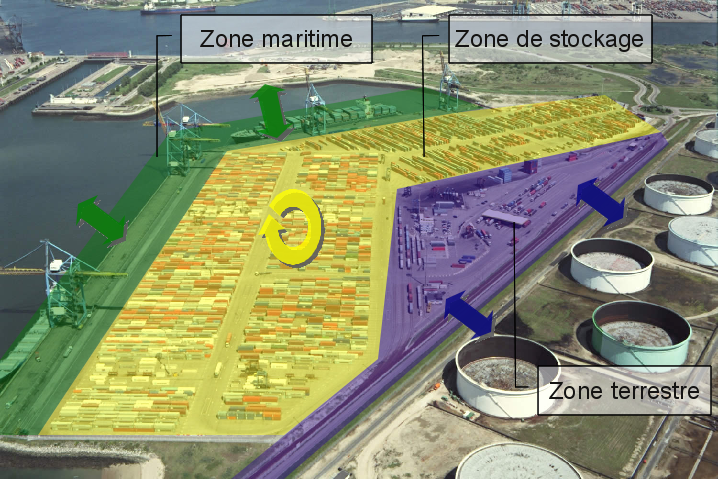
\includegraphics[width=0.5\textwidth]{chapitres/application/3zonesDuTN.png}
 \caption{Les 3 principales zones d'échange du Terminal de Normandie}
 \end{center}
\end{figure}

La zone de stockage est divisée en blocs. Chaque bloc comporte une série de travées où sont empilés les conteneurs. La hauteur maximale d'empilement varie en fonction des terminaux. Il y a 3 étages de conteneurs dans la zone de stockage des terminaux du port du Havre.
La zone des trains comporte plusieurs rangées de rails souvent entrecoupées par des routes afin de permettre aux engins de manutention de passer sans devoir faire le tour du train entier.
La zone des camions est constituée à l'entrée du terminal par des guichets où les conducteurs annoncent leur arrivée aux portes du terminal et leur ordre de chargement/livraison. Puis à l'intérieur du terminal des zones camions sont réparties afin d'accueillir les véhicules en attente de (dé)chargement.
La zone des quais comporte des portiques, le plus souvent mobiles permettant de décharger les conteneurs des navires sur les quais ou inversement de charger les conteneurs des quais sur les navires. Il est possible également que des camions se stationnent sous un portique afin de recevoir directement un conteneur du navire déchargé, ou de décharger son conteneur directement dans le navire.

\subsection{Engins de manutention}

Dans \cite{Steenken2004}, Steenken et al. distinguent 2 catégories de véhicules pouvant être rencontrés au sein d'un terminal à conteneurs : d'une part les véhicules des clients (trains, camions et navires) et d'autres part les engins de manutention du terminal.
Le transport des conteneur au sein du terminal peut être soit vertical, soit horizontal. Le transport vertical concerne les opération de levage et de dépose des conteneurs. Les engins concernés sont les portiques de quai ou de stockage. Ces engins sont la plupart du temps mobiles (soit sur rail, soit sur pneus) ce qui permet de les déplacer le long du quai ou le long des travées de stockage (voir fig. \ref{fig:portiqueBarge}. 

\begin{figure}[ht]
 \begin{center}
  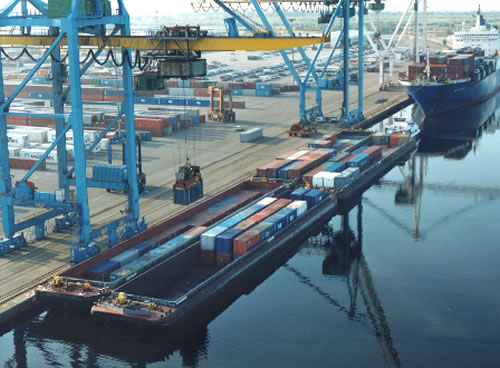
\includegraphics[width=0.5\textwidth]{chapitres/application/portique_barge.jpg}
  \caption{Portique du port du Havre, mobile sur rail, effectuant le déchargement d'une barge (source : \url{http://www.t-n.fr})}
  \label{fig:portiqueBarge}
 \end{center}
\end{figure}

Au contraire, le transport horizontal concerne les véhicules capable de déplacer un conteneur d'un endroit à un autre à l'intérieur du terminal. Les conteneurs doivent ainsi être déplacés entre la zone des camions et le yard, entre la zone des trains et le yard ainsi qu'entre les quais et le yard (et réciproquement du yard vers les zones des camions, trains et navires).
Il existe à l'heure actuelle deux procédés de gestion de ces déplacement : les véhicules passifs et les véhicules actifs.
Les véhicules actifs représente le procédé le plus moderne et consiste à utiliser des véhicules automatiques capables de transporter des conteneurs entre les différentes zones de manutention. Un système de câbles permet de délimiter les couloirs de circulation de ces engins qui sont ensuite capable de s'orienter automatiquement. Ces véhicules sont dis passifs car ils ne sont pas autonomes dans le sens où il ne sont pas capables de charger ou décharger un conteneur par eux-même. Ils doivent attendre d'être chargés ou déchargés par une grue. Ainsi, ces véhicules requirent la présence de portiques dans toutes les zones du terminal. Dans les ports utilisant cette technologie, des portiques sont utilisés pour empiler et dépiler les conteneurs des travées. Les AGV se garent sous le portique afin d'être chargés ou déchargés.

\begin{figure}[ht]
 \label{fig:AGV}
 \begin{center}
 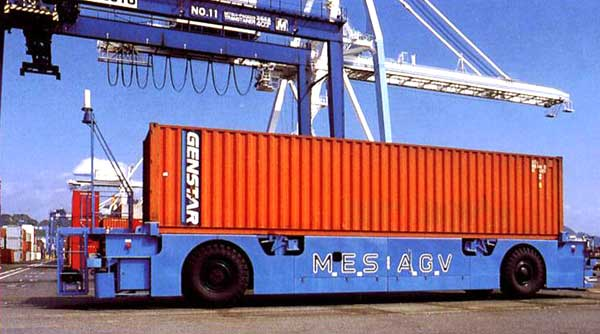
\includegraphics[width=0.5\textwidth]{chapitres/application/agv.png}
 \caption{Automated Guided Vehicle (AGV) de marque MES (source : mescranes.com)}
 \end{center}
\end{figure}

Les véhicules actifs d'autre part, consiste plus traditionnellement à utiliser des véhicules pilotés par des opérateurs et capable à la fois de transporter et de charger ou décharger un conteneur sans l'aide d'un portique. Il existe trois principaux engins de ce type : 
\begin{itemize}
 \item \textit{Forklift Truck} (chariots élévateurs) : ces chariots élévateurs permettent uniquement de manipuler des conteneurs vides. Ils servent donc à déplacer ces conteneurs dans une partie particulière du terminal où ils sont stockés;
 \item \textit{Reach Stacker }(chariots empileurs) : ces chariots sont utilisés pour charger et décharger les trains. La prise se fait par le côté, ce qui reprend l'avantage du chariot élévateur mais en permettant de soulever une charge beaucoup plus lourde;
 \item \textit{Straddle Carrier} (chariots cavaliers) : ces chariots sont les plus puissants. La prise se fait par le dessus. Ils sont capable d'enjamber une pile de conteneurs de 3 étages et permettent ainsi de se déplacer dans les travées.
\end{itemize}

Ce sont ces véhicules qui sont utilisés pour la manutention des conteneurs au sein des terminaux du port du Havre. Certains chariots sont capable d'adapter dynamiquement la longueur de leur pince afin de s'adapter aux différents types de conteneurs. D'autres chariots nécessitent de rentrer au dépôt afin qu'un mécanicien modifie l'écartement des pinces.
\begin{figure}[ht]
 \label{fig:enginsManutention}
 \begin{center}
 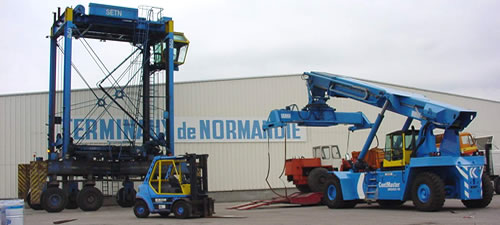
\includegraphics[width=0.5\textwidth]{chapitres/application/enginsTN.png}
 \caption{Engins de manutention utilisés par les Terminaux de Normandie (de gauche à droite) : chariot cavalier, chariot élévateur et chariot empileur (source : \url{http://www.t-n.fr)}}
 \end{center}
\end{figure}

\begin{figure}[ht]
 \label{fig:sc}
 \begin{center}
  \begin{tabular}{ccc}
	  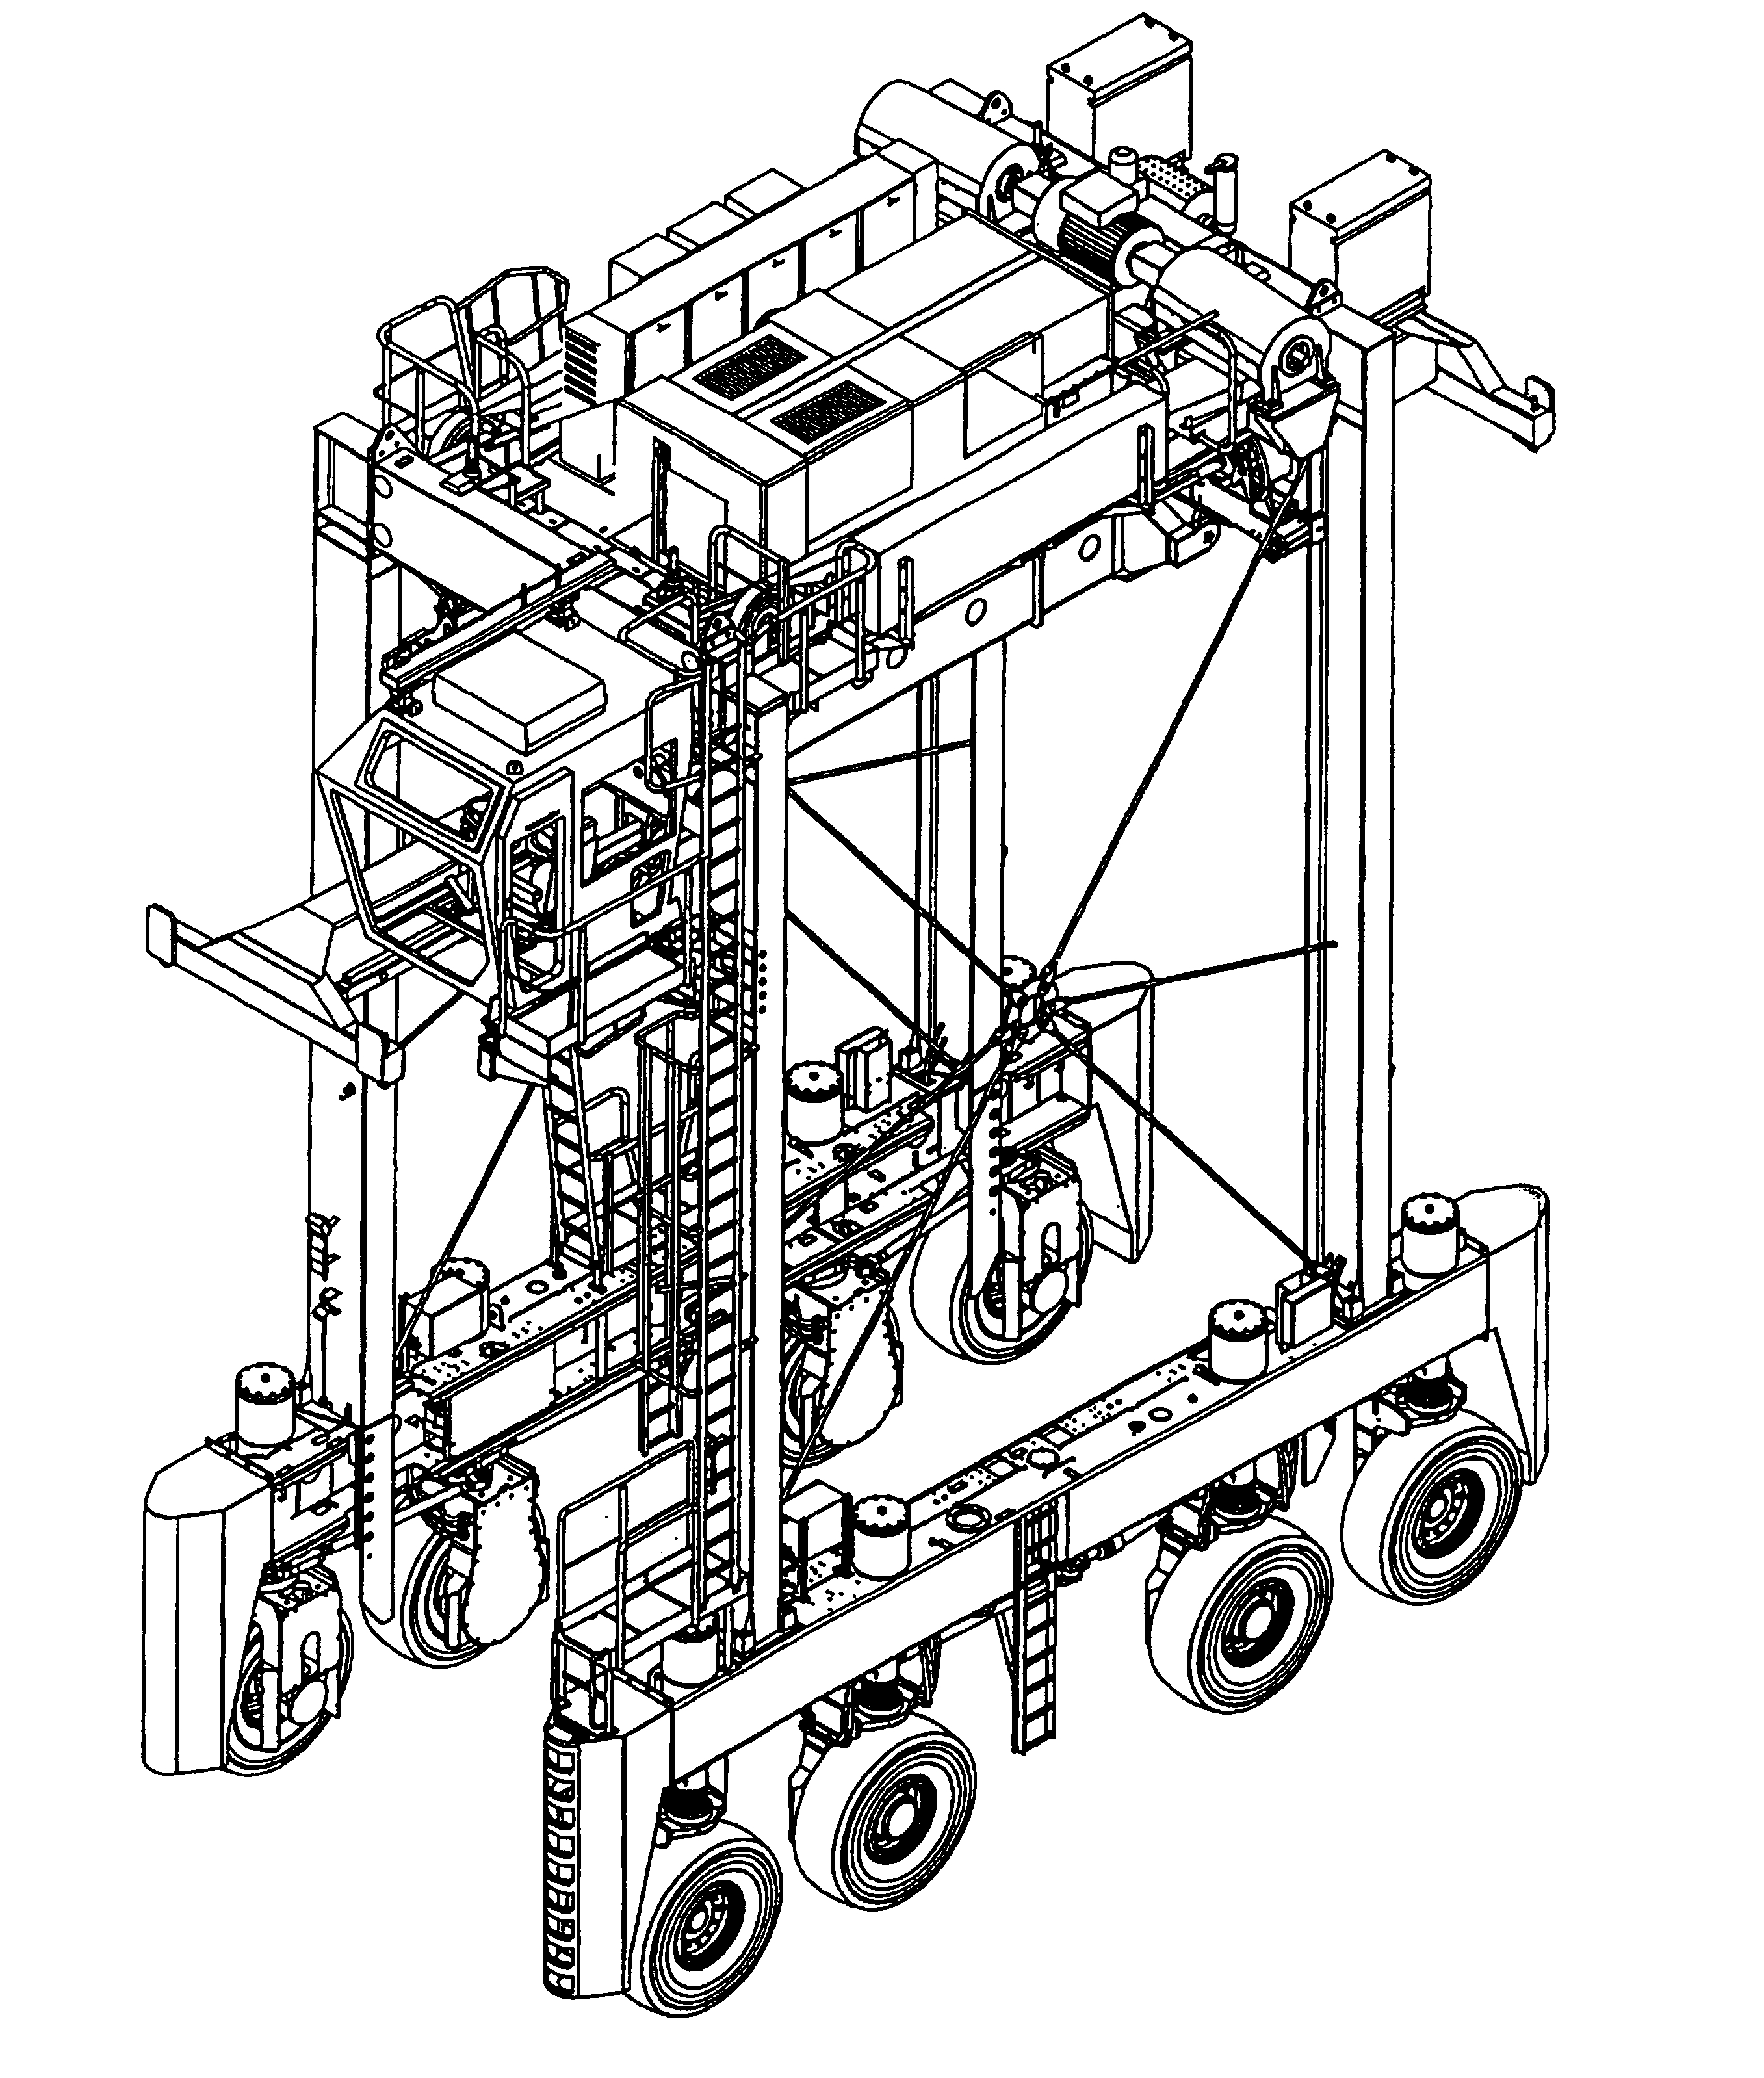
\includegraphics[height=3.5cm]{chapitres/application/schema_sc.jpg} & 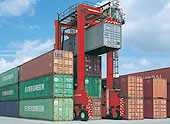
\includegraphics[height=3.5cm]{chapitres/application/tn-straddle-carriers.jpg} & 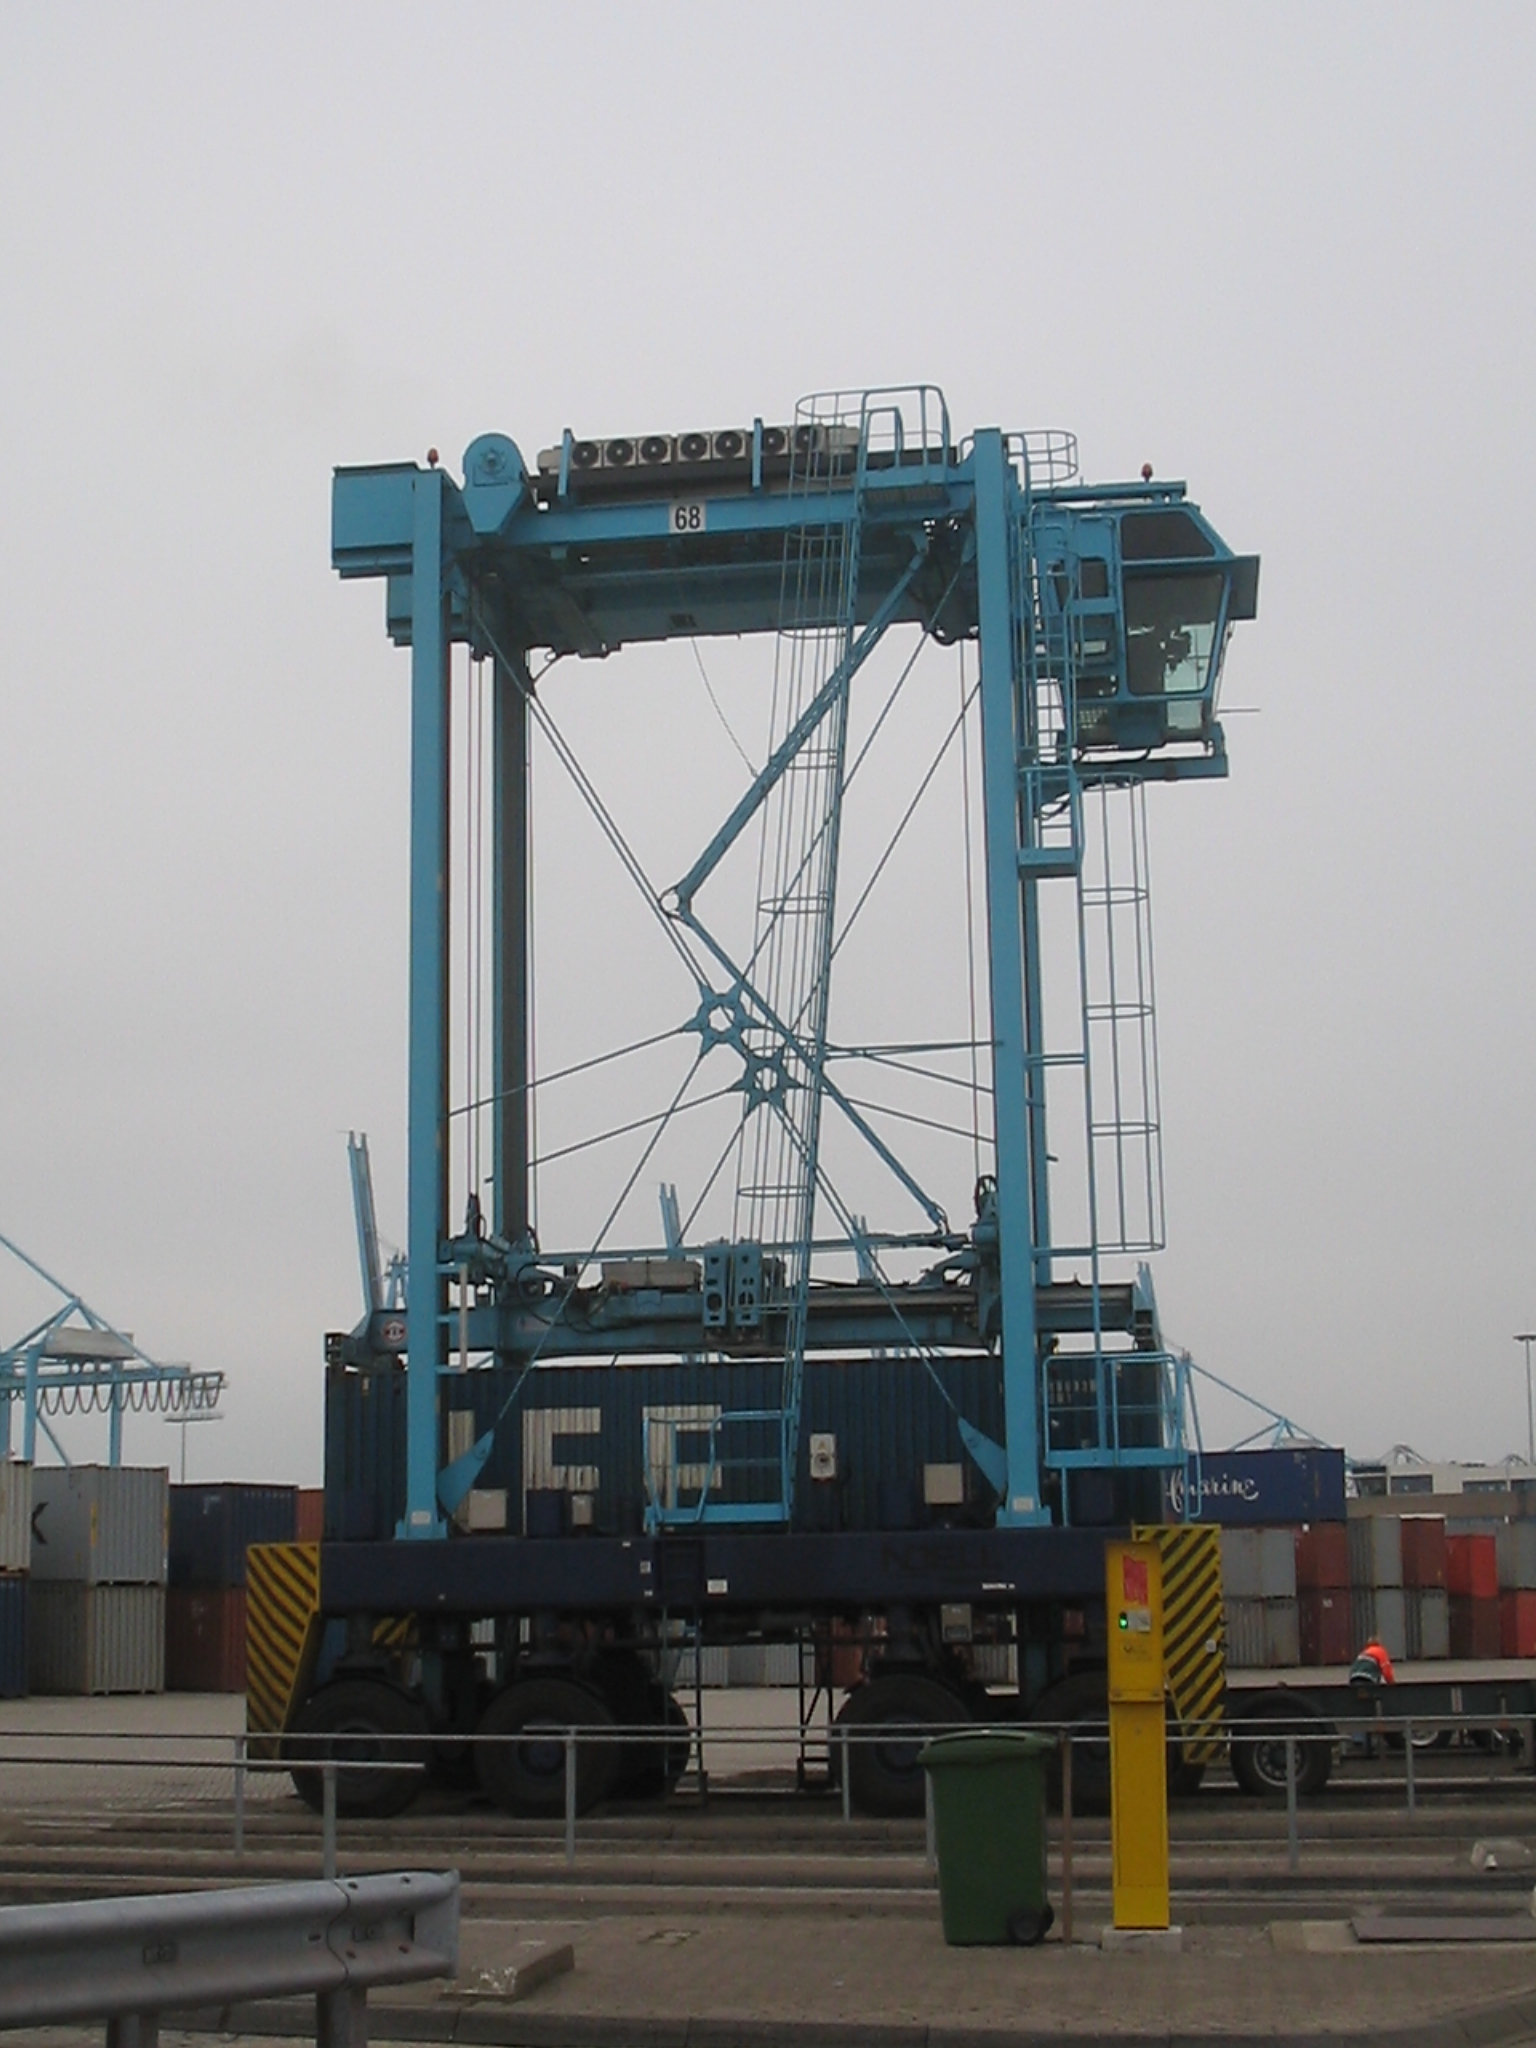
\includegraphics[height=3.5cm]{chapitres/application/containerlift_straddle_carrier.jpg}
  \end{tabular}
 \end{center}
  \caption{Chariots cavaliers}
\end{figure}

Cette thèse prend racine dans le contexte portuaire local et c'est pourquoi il ne sera question que de l'optimisation des déplacement des chariots et non pas des véhicules automatiques. Il est à noter qu'il ne sera fait référence qu'aux chariots cavaliers dans la suite de ce manuscrit tout en gardant à l'idée que les mêmes procédés s'appliquent également aux autres chariots (\textit{forklift trucks} et \textit{reach stackers}).

\subsection{Réseau routier}

Les différents blocs du terminal sont reliés grâce à un réseau constitué de routes et de carrefours. Ce réseau peut être modélisé par un graphe orienté $G=(V,A)$ où $V$ est l'ensemble des carrefours et où $A$ est l'ensemble des routes. Les travées de conteneurs constituent des routes praticables par les chariots cavaliers. Cependant, le fait d'enjamber les conteneurs rend impossible à deux chariots de se croiser ou de se doubler dans une même travée. L'espacement entre deux travée peut de même empêcher deux chariot de se croiser dans deux travées connexes. Ces routes spécifiques peuvent être modélisées par des arcs First-In-First-Out (voir \cite{Orda1990}). Ces arcs garantissent que le premier véhicule utilisant l'arc sera le premier à en ressortir.
Cette spécificité des arcs FIFO a pour conséquence de provoquer des temps d'attente potentiels des chariots en entrée de travée. Ceci peut avoir un impact lourd sur les performances du routage des chariots et doit être pris en compte avec attention. En effet, certaines zones du réseau routier du terminal sont faiblement connexe et peuvent être rapidement saturées. Un routage efficace consistera principalement à ne plus considérer la distance parcourue comme unique critère d'optimisation mais également le temps de parcours.

\subsection{Activités des chariots cavaliers}

Les chariots cavaliers sont utilisés pour déplacer les conteneurs à l'intérieur du terminal. Chaque déplacement est appelé ``mission''. Lorsqu'un chariot n'effectue aucune mission, on dit qu'il est ``libre``. Il stationne alors dans une zone spécifique du terminal appelée ''dépôt``. 
Chaque mission comporte 4 phases. D'abord une phase de déplacement vers le point de collecte, puis la phase de chargement du conteneur sur le chariot, ensuite une nouvelle phase de déplacement mais cette fois vers l'emplacement de livraison, et enfin, la phase de déchargement du conteneur du chariot.

\subsubsection{Les types de missions}
Une mission peut être de 4 types :
\begin{itemize}
 \item Entrée : un conteneur doit être stocké dans le yard
 \item Sortie : un conteneur doit être amené du yard vers une zone d'échange (camion, train ou quai)
 \item Transbordement : un conteneur doit être déplacé d'un quai à un autre
 \item Réorganisation : un conteneur doit être déplacé à l'intérieur du yard
\end{itemize}

La première catégorie de mission concerne le déchargement des camions, trains ou porte-conteneurs. Les chariots se rendent sur l'emplacement de collecte du conteneur (au dessus de la remorque du camion, du wagon, ou sous le portique de quai), prennent le conteneur concerné par la mission, puis se dirigent vers l'emplacement de livraison à l'intérieur du yard et y dépose le conteneur.
La seconde catégorie de mission concerne l'opération inverse, c'est à dire le chargement des camions, trains ou porte-conteneurs. Les chariots se rendent sur l'emplacement de collecte du conteneur dans le yard, prennent le conteneur concerné, puis se dirigent vers l'emplacement de livraison (au dessus de la remorque du camion, du wagon, ou sous le portique de quai) et dépose le conteneur sur le sol dans le cas d'un quai, ou sur la remorque du camion, ou encore sur le wagon du train.
La troisième opération concerne le chargement des conteneurs d'un navire sur un autre porte-conteneurs. Le chariot doit alors récupérer le conteneur de la mission sous le portique de quai, puis se diriger vers le portique de chargement du navire à charger et y déposer le conteneur qui sera acheminé à bord par la grue.
Enfin, l'opération de réorganisation consiste à déplacer les conteneurs à l'intérieur de la zone de stockage afin de préparer l'arrivée (la sortie) de conteneurs du terminal. Cette opération permet d'éviter d'avoir au dernier moment à dépiler un certains nombre de conteneurs pour accéder à un conteneur en bas d'une pile par exemple.

\subsubsection{Fenêtres de temps}

Deux fenêtres de temps sont attribuées à chaque mission. Ces fenêtres indiquent les périodes de temps à respecter d'une part pour collecter le conteneur, et d'autre part pour le livrer.
Si un chariot cavalier arrive avant le début de la fenêtre de temps, il devra attendre. S'il arrive après la fin de la fenêtre de temps, c'est le véhicule client (camion, train, porte-conteneur) qui devra attendre. Cette attente des clients peut provoquer des frais supplémentaires pour le terminal qui devra payer des pénalités de retard. Les fenêtres de temps peuvent être ainsi strictes (\textit{hard}) ou lâches (\textit{soft}). 
Ainsi, les fenêtres impliquant un client seront strictes afin de réduire les coûts, alors que les fenêtres de temps n'impliquant que des véhicules du terminal seront molles. En effet, lors d'une mission de chargement de camion par exemple, la collecte du conteneur à livrer se situe dans le yard. Si le chariot manque sa fenêtre de temps pour la collecte, cela n'entraînera pas de pénalité à payer pour le 
terminal.
La fenêtre de collecte est donc molle. En revanche la livraison du conteneur concerne un camion et le non respect de la fenêtre de temps entraînera des frais de pénalité à payer pour le terminal. La fenêtre de temps de livraison sera donc stricte.

\subsubsection{Objectifs des chariots cavaliers}

%Dire combien un chariot consomme de carburant
%Dire combien coute un chariot cavalier
Un chariot cavalier mesure environ 15 mètres de haut pour 10 mètres de long et 5 mètres de large et pèse près de 60 tonnes à vide.
Capable de déplacer une charge de 50 tonnes à la vitesse de 20 km/h, un chariot peut se déplacer à vide jusqu'à 40 km/h.
Sa consommation de carburant dépasse les 20 L/h. 

\begin{figure}[ht]
  \begin{center}
   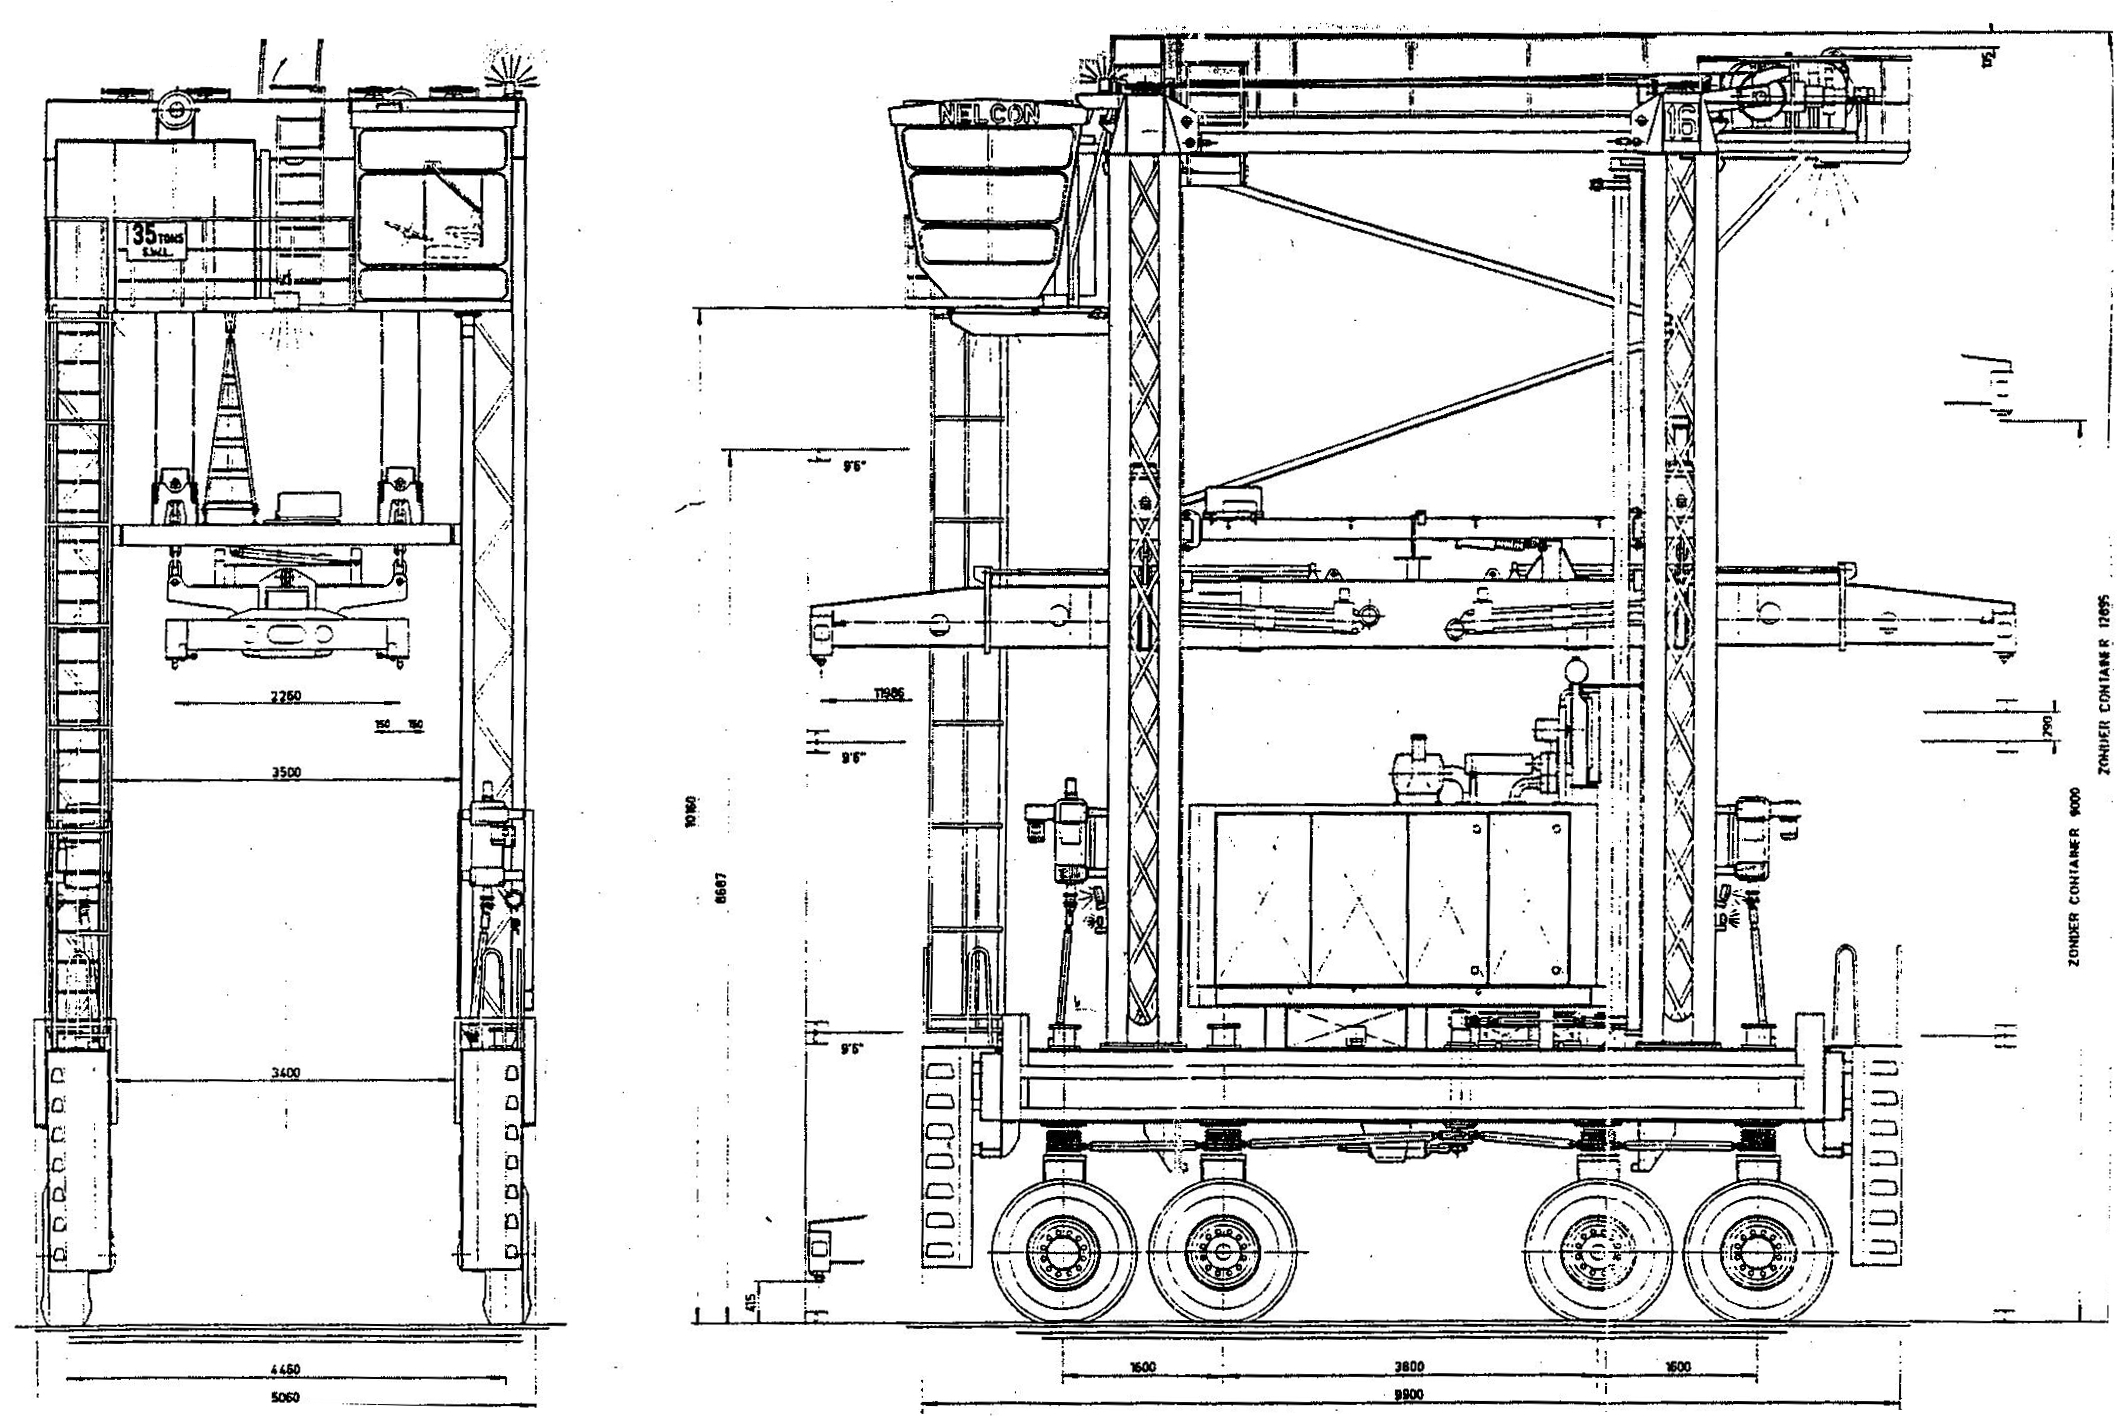
\includegraphics[width=0.9\textwidth]{chapitres/application/planSC.jpg}
   \caption{Plan d'un chariot cavalier utilisé par le port du Havre dans les années 1990}
   \label{fig:application:planSC}
  \end{center}
\end{figure}

Ces caractéristiques techniques font qu'un chariot est extrêmement coûteux à la fois à l'achat (plus de 800000 \geneuro) et à l'utilisation (voir \cite{Huang2003}).
De plus, le pilotage de ces engins requiert une main d'\oe uvre de haute qualité dotée d'une grande précision afin de réaliser des manœuvres complexe impliquant de très lourdes charges en toute sécurité.
Afin de conserver une concentration et une précision accrue, ces pilotes ne peuvent conduire un chariot cavalier que pendant une période donnée dépendant du terminal concerné. Puis une phase de repos doit être respectée avant que le conducteur puisse reprendre son travail. Pour le terminal, cette main d'\oe uvre est un coût conséquent et doit être gérée de façon optimale.

À l`échelle du terminal, l'objectif est comme pour toute entreprise de services de dégager des profits.
Il est donc important de chercher à réduire les coûts et ceci peut être réalisé en partie en minimisant le nombre de chariots à utiliser et cherchant à réduire au minimum les distances parcourues par la flotte de chariots cavaliers.

À l'échelle d'un chariot cavalier, la qualité de service offerte au clients dépendra principalement de deux facteurs. D'une part, le soin pris par le conducteur du chariot pour charger/décharger un conteneur, et surtout d'autre part le respect des fenêtres de temps de la mission. Les caractéristiques temporelles évoquées dans le paragraphe précédent doivent être prisent en compte lors du calcul de l'ordonnancement des missions.

Pour toutes ces raisons et à la fois à l'échelle du terminal et à l'échelle des chariots cavaliers, les objectifs sont double. Pour le terminal, il est nécessaire de minimiser la taille de la flotte d'engins de manutention, de mains d’œuvre... tout en maximisant la qualité de service. À l'échelle des chariots cavaliers, les objectifs sont de minimiser la distance parcourue tout en minimisant le dépassement des fenêtres de temps.

\subsection{Le Terminal de Normandie}

Le Terminal de Normandie est l'un des terminaux du port du Havre. 
Il est situé dans l'estuaire de la seine dans un bassin à marée et est délimité au Nord par deux quais. Le quai d'Asie (au Nord-Ouest) et le quai d'Osaka (au Nord-Est) offrant ainsi à tous les deux 1075 mètres d'accostage et une profondeur de 14 mètres.
La superficie totale du terminal est de 40 Hectares et sa capacité annuelle est de 450000 EVP.

\begin{figure}[ht]
  \begin{center}
    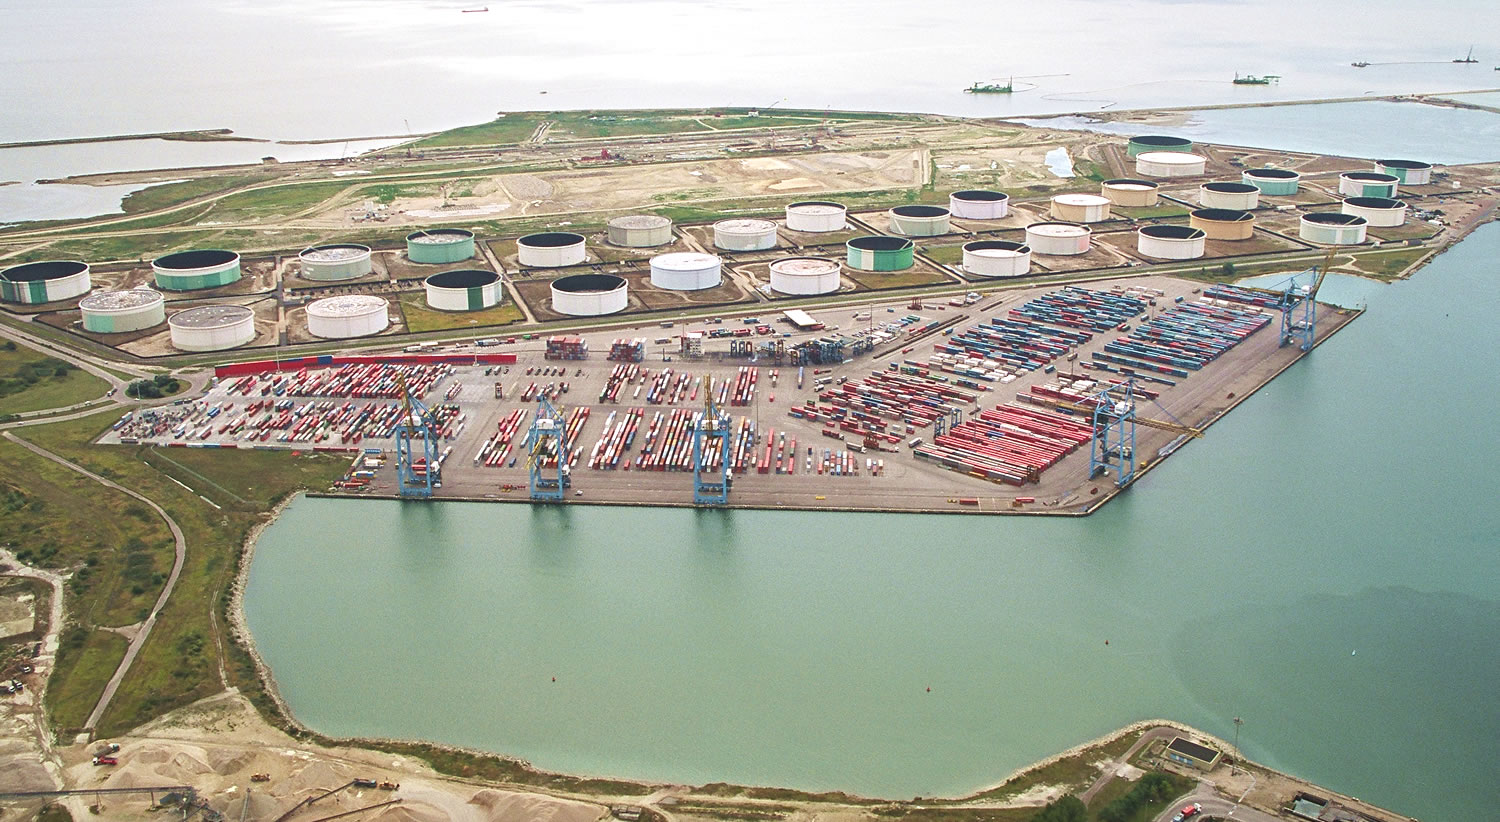
\includegraphics[width=0.8\textwidth]{chapitres/application/terminalDeNormandie.jpg}
    \caption{Terminal de Normandie, Port Autonome du Havre (source : \url{http://www.t-n.fr})}
    \label{fig:TN}
 \end{center}
\end{figure}

Le graphe représentant le réseau routier interne du terminal comporte 1170 sommets, 170 routes et 531 travées pour un total de 3500 emplacements de stockage de conteneurs. La zone de stockage est composée de 12 blocs permettant aisément de disposer les conteneurs à proximité de leur futur zone de transit. La zone des trains comporte 3 voies ferrées différentes entrecoupées sur certaines parties afin de permettre le passage des engins de manutention. Enfin, il existe 3 différentes zones de collecte et de livraison pour les camions.

Ce terminal a été créé en 1990 afin de contenir le flux d'échanges de conteneurs qui n'a cessé d'augmenter de façon de plus en plus importante. À l'époque de sa construction, ce terminal était capable d'accueillir les plus grands navires porte-conteneurs. En revanche, de nouveaux navires géants aux dimensions impressionnantes ont été construits depuis et sont gérés dans un autre terminal du port du Havre construit plus récemment.

\begin{figure}[ht]
  \begin{center}
    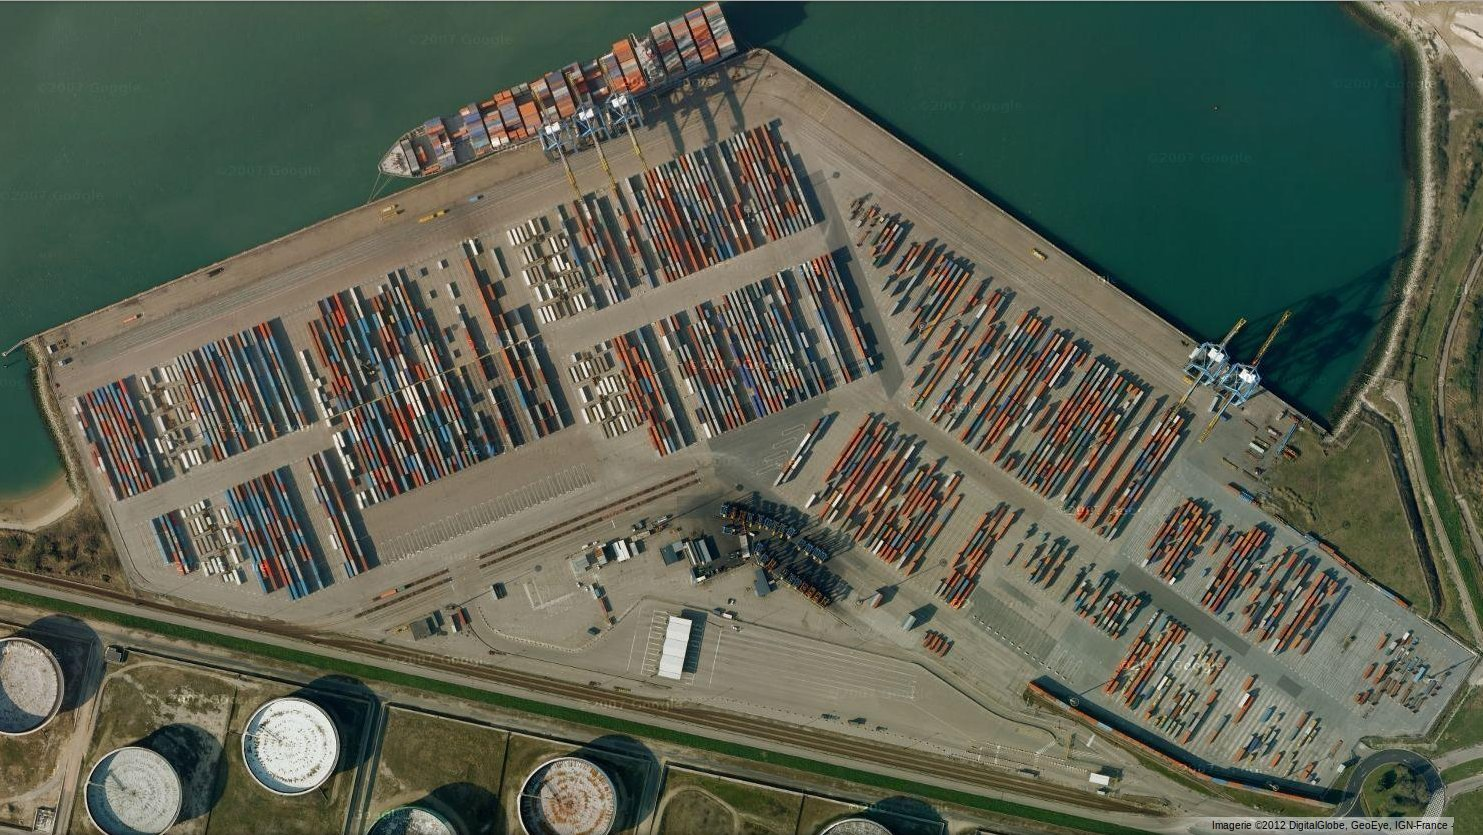
\includegraphics[width=0.8\textwidth]{chapitres/application/terminalDeNormandieGoogleMaps.jpg}
    \caption{Image satellite du Terminal de Normandie, Port Autonome du Havre (source : Google Maps)}
    \label{fig:TNGoogle}
 \end{center}
\end{figure}

5 portiques de quais et une vingtaine de chariots cavaliers assurent la manutention des conteneurs à l'intérieur du terminal où aucun portique n'est utilisé dans la zone de stockage. Les chariots cavaliers sont les seuls engins autorisés à circuler et à manipuler des conteneurs dans les blocs de travées. La régulation du trafic à l'intérieur du terminal est donc un point critique concernant la performance du terminal c'est pourquoi une bonne gestion des engins de manutention est primordiale afin d'assurer une qualité de service suffisante aux clients du terminal.\\


%détailler dans la partie SIMULATEUR la modélisation du terminal ainsi que l'acquisition des données...
